% HMC Math dept HW template example
% v0.04 by Eric J. Malm, 10 Mar 2005
\documentclass[10pt,a4paper,boxed]{hmcpset}

% set 1-inch margins in the document
% \usepackage[margin=1in]{geometry}
\usepackage{enumerate}
\usepackage{tikz}
\usetikzlibrary{positioning}
\usepackage{pgfplots}
\usepackage{amsmath}
\usepackage{amsfonts}
\usepackage{amssymb}

% include this if you want to import graphics files with /includegraphics
\usepackage{graphicx}

\renewcommand*{\familydefault}{\sfdefault}
\newcommand{\vect}[1]{\mathbf{#1}}

\tikzset{node distance=2cm, inner/.style={draw,circle}, leaf/.style={draw,rectangle}}

% info for header block in upper right hand corner
\name{Group 6: Timm Behner, Philipp Bruckschen, Patrick Kaster, Markus Schwalb}
\class{MA-INF 4111 - Intelligent Learning and Analysis Systems: Machine Learning}
\assignment{Exercise Sheet 2}
% \duedate{09/03/2004}

\begin{document}

%\problemlist{Rudin 3.5, Saff and Snider 1.5.11, 1.7.5ad,\\Dummit and Foote 1.1.25, Logan 1.8.6}
\begin{problem}[2. Decision Tree Representations of Boolean Functions]
\end{problem}
\begin{solution}
	\begin{enumerate}
		\item $f(A,B) = A \vee B$ \hfill \\[1em]
			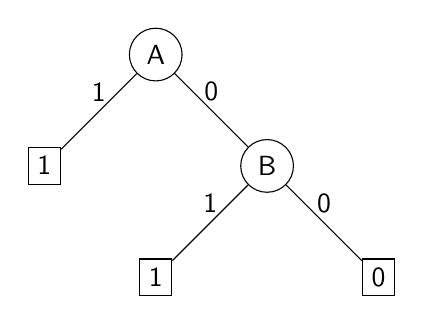
\begin{tikzpicture}
				\node[inner] (A) {A};
				\node[inner] (B) [below right of=A] {B};
				\node[leaf]  (L1) [below left of=A] {1};
				\node[leaf]  (L2) [below left of=B] {1};
				\node[leaf]  (L3) [below right of=B] {0};

				\path[draw]
					(A) -- node[above] {0} (B)
					(A) -- node[above] {1} (L1)
					(B) -- node[above] {1} (L2)
					(B) -- node[above] {0} (L3);
			\end{tikzpicture}

		\item $f(A,B) = A \wedge B$ \hfill \\[1em]
			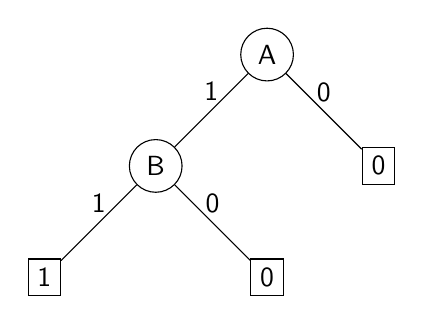
\begin{tikzpicture}
				\node[inner] (A) {A};
				\node[inner] (B) [below left of=A] {B};
				\node[leaf]  (L1) [below right of=A] {0};
				\node[leaf]  (L2) [below left of=B] {1};
				\node[leaf]  (L3) [below right of=B] {0};

				\path[draw]
					(A) -- node[above] {1} (B)
					(A) -- node[above] {0} (L1)
					(B) -- node[above] {1} (L2)
					(B) -- node[above] {0} (L3);
			\end{tikzpicture}

		\item  $f(A,B) = A \oplus B$ \hfill \\[1em]
			\begin{tikzpicture}
				\node[inner] (A) {A};
				\node[inner] (B1) [below left=of A,xshift=-1cm] {B};
				\node[inner] (B2) [below right=of A,xshift=1cm] {B};
				\node[leaf]  (L1) [below left=of B1] {0};
				\node[leaf]  (L2) [below right=of B1] {1};
				\node[leaf]  (L3) [below left=of B2] {1};
				\node[leaf]  (L4) [below right=of B2] {0};

				\path[draw]
				(A) -- node[above] {1} (B1)
				(A) -- node[above] {0} (B2)
				(B1) -- node[above] {1} (L1)
				(B1) -- node[above] {0} (L2)
				(B2) -- node[above] {1} (L3)
				(B2) -- node[above] {0} (L4)
				;

			\end{tikzpicture}

		\item $f(A,B,C,D) = (A \vee B) \wedge (C \vee \neg D \vee E)$ \hfill \\[1em]

			\begin{tikzpicture}
				\node[inner] (A) {A};
				\node[inner] (C1) [below left=of A,xshift=-2cm] {C};
				\node[inner] (B) [below right=of A,xshift=2cm] {B};
				\node[inner] (D1) [below right=of C1,xshift=-0.5cm] {D};
				\node[inner] (E1) [below left=of D1] {E};
				\node[inner] (C2) [below left=of B] {C};
				\node[inner] (D2) [below right=of C2] {D};
				\node[inner] (E2) [below left=of D2] {E};

				\node[leaf] (L1) [below left=of C1] {1};
				\node[leaf] (L2) [below left=of E1] {1};
				\node[leaf] (L3) [below right=of E1] {0};
				\node[leaf] (L4) [below right=of D1] {1};

				\node[leaf] (L5) [below left=of C2] {1};
				\node[leaf] (L6) [below left=of E2] {1};
				\node[leaf] (L7) [below right=of E2] {0};
				\node[leaf] (L8) [below right=of D2] {1};

				\node[leaf] (L9) [below right=of B] {0};

				\path[draw]
				(A) -- node[above] {1} (C1)
				(A) -- node[above] {0} (B)
				(B) -- node[above] {1} (C2)
				(B) -- node[above] {0} (L9)

				(C1) -- node[above] {1} (L1)
				(C1) -- node[above] {0} (D1)
				(D1) -- node[above] {0} (L4)
				(D1) -- node[above] {1} (E1)
				(E1) -- node[above] {1} (L2)
				(E1) -- node[above] {0} (L3)

				(C2) -- node[above] {1} (L5)
				(C2) -- node[above] {0} (D2)
				(D2) -- node[above] {0} (L8)
				(D2) -- node[above] {1} (E2)
				(E2) -- node[above] {1} (L6)
				(E2) -- node[above] {0} (L7)
				;
			\end{tikzpicture}

	\end{enumerate}
\end{solution}

\begin{problem}[3. Properties of the Entropy]
\end{problem}
\begin{solution}
	\begin{enumerate}[(i)]	
		\item \label{task1}
		\begin{alignat}{1}
			H(X) = H\left(p_{1}\ldots p_{n}\right) = & \sum_{i=1}^{n}-p_{i}\log_{2}p_{i} \nonumber \\ 
				 = & \sum_{i=1}^{n}p_{i}\log_{2}\frac{1}{p_{i}} \nonumber \\
				 = & \mathbb{E}\left[\log_{2}\left(X\right)\right]\leq\log_{2}\left(\mathbb{E}\left[X\right]\right) \label{eq:concavelog} \\
				 = & \log_{2}\left(\sum_{i=1}^{n}p_{i}\frac{1}{p_{i}}\right) \nonumber \\
				 = & \log_{2}n \nonumber
		\end{alignat}
		
		We used the well known concavity of the logarithm in applying Jensen's inequality in (\ref{eq:concavelog}).
		
		\item
		\begin{alignat*}{1}
			\mathrm{Gain}\left(X\vert Y\right)     = & H\left(X\right)-H\left(X|Y\right)\\
												   = &\sum_{X}-P\left(X\right)\log_{2}P\left(X\right)-\sum_{v\in\mathrm{value}(Y)}P\left(Y=v\right)H\left(X\vert Y=v\right)\\
											       = & \sum_{X}-P\left(X\right)\log_{2}P\left(X\right)\\
											       - & \sum_{v\in\mathrm{value}(Y)}P\left(Y=v\right)\sum_{X}\left(-P\left(X\vert Y=v\right)\log_{2}P\left(X\vert Y=v\right)\right)\\
		\end{alignat*}
		
		\begin{alignat*}{1}
			\Leftrightarrow\mathrm{-Gain}\left(X\vert Y\right) = & \sum_{X}P\left(X\right)\log_{2}P\left(X\right)\\
															   - & \sum_{v\in\mathrm{value}(Y)}P\left(Y=v\right)\sum_{X}P\left(X\vert Y=v\right)\log_{2}P\left(X\vert Y=v\right)\\
 												   = & \sum_{X}\sum_{v\in\mathrm{value}(Y)}P\left(X,Y=v\right)\log_{2}P\left(X\right)\\
 												   - & \sum_{v\in\mathrm{value}(Y)}\sum_{X}P\left(Y=v\right)P\left(X\vert Y=v\right)\log_{2}P\left(X\vert Y=v\right)\\
												   = & \sum_{X}\sum_{v\in\mathrm{value}(Y)}P\left(X,Y=v\right)\log_{2}P\left(X\right)\\
												   - & \sum_{v\in\mathrm{value}(Y)}\sum_{X}P\left(X,Y=v\right)\log_{2}P\left(X\vert Y=v\right)\\
		\end{alignat*}
		
		\begin{alignat}{1}
												   = & \sum_{X}\sum_{v\in\mathrm{value}(Y)}P\left(X,Y=v\right)\left(\log_{2}P\left(X\right)-\log_{2}P\left(X\vert Y=v\right)\right) \nonumber\\
												   = & \sum_{X}\sum_{v\in\mathrm{value}(Y)}P\left(X,Y=v\right)\left(\log_{2}\left(\frac{P\left(X\right)}{P\left(X\vert Y=v\right)}\right)\right)\nonumber\\
												   = & \sum_{X}\sum_{v\in\mathrm{value}(Y)}P(Y=v)P\left(X|Y=v\right)\left(\log_{2}\left(\frac{P\left(X\right)}{P\left(X\vert Y=v\right)}\right)\right)\nonumber\\
												   = & \sum_{v\in\mathrm{value}(Y)}P(Y=v)\sum_{X}P\left(X|Y=v\right)\left(\log_{2}\left(\frac{P\left(X\right)}{P\left(X\vert Y=v\right)}\right)\right)\label{eq:J1}\\
												\leq & \sum_{v\in\mathrm{value}(Y)}P(Y=v)\left(\log_{2}\left(\sum_{X}\frac{P\left(X\right)P\left(X|Y=v\right)}{P\left(X\vert Y=v\right)}\right)\right)\label{eq:J2}\\
												\leq & \log_{2}\left(\sum_{v\in\mathrm{value}(Y)}\sum_{X}\frac{P\left(X\right)P\left(X|Y=v\right)P(Y=v)}{P\left(X\vert Y=v\right)}\right)\label{eq:J3}\\
												   = & \log_{2}\left(\sum_{v\in\mathrm{value}(Y)}P(Y=v)\sum_{X}P\left(X\right)\right)\nonumber \\
 												\leq & \log_{2}\left(\sum_{v\in\mathrm{value}(Y)}P(Y=v)\right)\nonumber\\
												   = & \log_{2}\left(1\right)=0 \nonumber
		\end{alignat}
		
		So we conclude: \[ \mathrm{-Gain}\left(X\vert Y\right) \leq \log_{2}\left(1\right) = 0 \Leftrightarrow \mathrm{Gain}\left(X\vert Y\right) \geq 0 \]
		We used Jensen's inequality from task (\ref{task1}) from equation (\ref{eq:J1}) to (\ref{eq:J2}) and again from (\ref{eq:J2}) to (\ref{eq:J3}).

	\end{enumerate}
	
\end{solution}


\end{document}
